\documentclass{article}

\usepackage[utf8]{inputenc}

\title{COMP 540 Assignment \#1}
\author{Yunda Jia\\Yu Wu}
\date{\today}
\usepackage{natbib}
\usepackage{graphicx}
\usepackage{geometry}
\usepackage{amsmath}
\usepackage{bm}
\usepackage{mathrsfs}
\usepackage{mathdots}
\usepackage{subfigure}
\usepackage{subfig}
\setcounter{section}{-1}
\geometry{left=2.0cm,right=2.0cm,top=2.0cm,bottom=2.0cm}

\begin{document}
\maketitle

\section{Background refresher(30 points)}
\begin{itemize}
	\item Plot the categorical distribution.\\
\begin{figure}[h!]
	\centering
	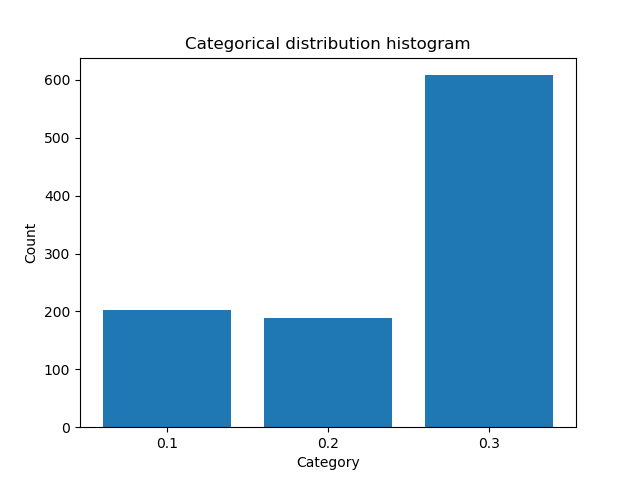
\includegraphics[scale = 0.5]{Categorical_distribution.png}
	\caption{Categorical distribution}
\end{figure}

\item Plot the Univariate normal distribution with mean of and standard deviation of 1.\\
\begin{figure}[h!]
	\centering
	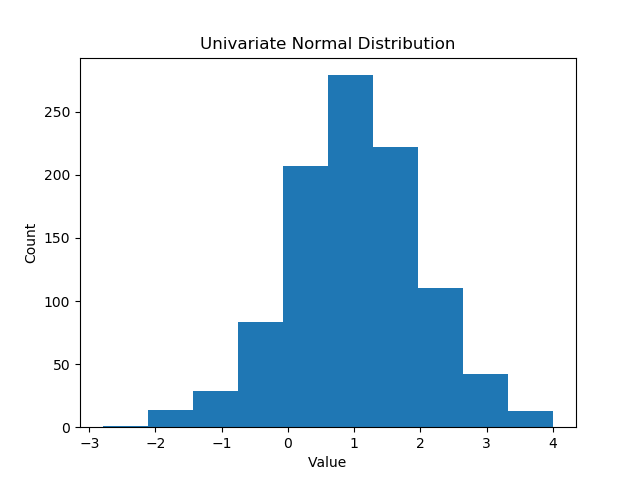
\includegraphics[scale = 0.5]{Univariate_distribution.png}
	\caption{Univariate Normal Distribution}
\end{figure}\\
\pagebreak
\item Produce a scatter plot of the samples for a 2-D Gaussian.\\
\begin{figure}[h!]
	\centering
	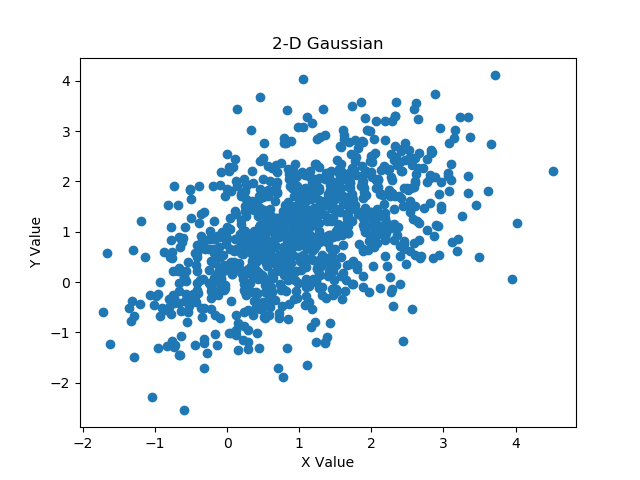
\includegraphics[scale = 0.7]{GaussianScatterPlot.png}
	\caption{Univariate Normal Distribution}
\end{figure}\\

\item Test mixture sampling code
Code can be seen in sampler.py. Mixture Gaussian plot is shown below\\
\begin{figure}[h!]
	\centering
	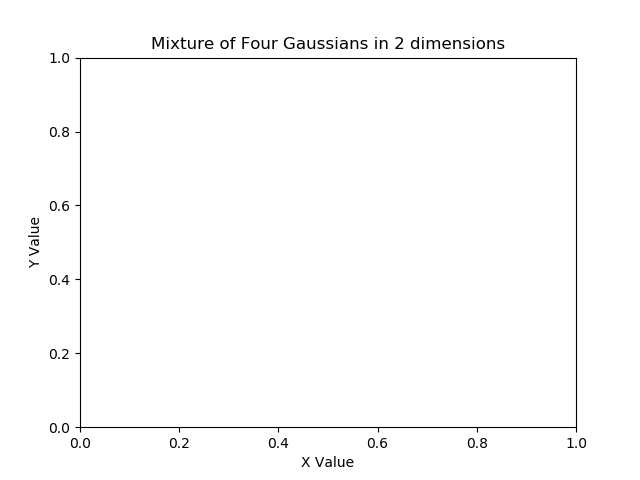
\includegraphics[scale = 0.7]{MixtureGaussians.png}
	\caption{Univariate Normal Distribution}
\end{figure}\\
\pagebreak
\item Prove that the sum of two independent Poisson random variables is also a Poisson random variable.\\
Suppose $X \sim \mathcal{P}(\lambda)$ and $Y \sim \mathcal {P}(\mu)$. Now Prove that $X + Y \sim \mathcal{P}(\lambda + \mu)$.\\

\begin{align*}
  P(X+ Y =k) &= \sum_{i = 0}^k P(X+ Y = k, X = i)\\
    &= \sum_{i=0}^k P(Y = k-i , X =i)\\
    &= \sum_{i=0}^k P(Y = k-i)P(X=i)\\
    &= \sum_{i=0}^k e^{-\mu}\frac{\mu^{k-i}}{(k-i)!}e^{-\lambda}\frac{\lambda^i}{i!}\\
   &= e^{-(\mu + \lambda)}\frac 1{k!}\sum_{i=0}^k \frac{k!}{i!(k-i)!}\mu^{k-i}\lambda^i\\
   &= e^{-(\mu + \lambda)}\frac 1{k!}\sum_{i=0}^k \binom ki\mu^{k-i}\lambda^i\\
   &= \frac{(\mu + \lambda)^k}{k!} \cdot e^{-(\mu + \lambda)}
\end{align*}
So $X + Y \sim \mathcal{P}(\lambda + \mu)$.\\
\item Find $\alpha, \mu_{1}$ and $\sigma_{1}$.\\
We have $X_{0}$ and $X_{1}$ be continuous random variables. If\\
\begin{align*}
    p(X_{0} = x_{0}) &= \alpha_{0}e^{-\frac{(x_{0} - \mu_{0})^2}{2\sigma_{0}^2}}\\
    P(X_{1} = x_{1}|X_{0} = x_{0}) &= \alpha_{1}e^{-\frac{(x_{1} - x_{0})^2}{2\sigma^2}}
\end{align*}\\
\begin{align*}
    p(X_{1} = x_{1}) &= \int P(X_{1} = x_{1}|X_{0} = x_{0}) \cdot p(X_{0} = x_{0}) d x_{0}\\
    &= \alpha_{0}\alpha_{1}\int e ^{-\frac{\sigma^2(x_{0} - \mu_{0})^2 + \sigma_{0}^2(x_{1} - x_{0})^2}{2\sigma_{0}^2\sigma^2}}d x_{0}\\
    &= \alpha_{0}\alpha_{1}\int e ^{-\frac{(\sigma^2 + \sigma_{0}^2)x_{0}^2 - 2(\sigma^2\mu_{0} + \sigma_{0}^2x_{1})x_{0} + \sigma^2\mu_{0}^2 + \sigma_{0}^2x_{1}^2}{2\sigma_{0}^2\sigma^2}}d x_{0}\\
    &= \alpha_{0}\alpha_{1}\int e^{-\frac{1}{2\sigma_{0}^2\sigma^2}[(\sqrt{\sigma^2 + \sigma_{0}^2}x_{0} - \frac{-\sigma^2\mu_{0} + \sigma_{0}^2x_{1}}{\sqrt{\sigma^2 + \sigma_{0}^2}})^2 + \sigma^2\mu_{0}^2 + \sigma_{0}^2x_{1}^2 - \frac{\sigma^2\mu_{0}^2 + \sigma_{0}^2x_{1}^2}{\sigma^2 + \sigma_{0}^2}]} d x_{0}\\
\end{align*}
Since \begin{align*}
    \int \frac{1}{\sqrt{2\pi \sigma}}e^{-\frac{(x - \mu) ^ 2}{2\sigma^2}}d x = 1
\end{align*}\\
\begin{align*}
    p(X_{1} = x_{1}) &= \frac{\alpha\alpha_{0}\sqrt{2\pi}\sigma\sigma_{0}}{\sqrt{\sigma^2 + \sigma_{0}^2}} e ^ {-\frac{1}{2\sigma_{0}^2\sigma^2}(\sigma^2\mu_{0}^2 + \sigma_{0}^2x_{1}^2 - \frac{\sigma^2\mu_{0}^2 + \sigma_{0}^2x_{1}^2}{\sigma^2 + \sigma_{0}^2})}\\
    &= \alpha e^{-\frac{(x_{1} - \mu_{0})^2}{2(\sigma^2 + \sigma_{0}^2)}}
\end{align*}
Thus we can solve that:\\
\begin{align*}
    \alpha &= \frac{\alpha\alpha_{0}\sqrt{2\pi}\sigma\sigma_{0}}{\sqrt{\sigma^2 + \sigma_{0}^2}}\\
    \mu_{1} &= \mu_{0}\\
    \sigma_{1} &= \sqrt{\sigma^2 + \sigma_{0}^2}
\end{align*}
\item Consider the vectors $\bm{u} = \begin{bmatrix}
	1&2
\end{bmatrix}^\mathrm{T}$ and $\bm{v} = \begin{bmatrix}
	2&3
\end{bmatrix}^\mathrm{T}$. Define the matrix $\bm{M} = \bm{u}\bm{v}^\mathrm{T}$. Compute the eigenvalues and eigenvectors of $\bm{M}$.\\
\begin{align*}
	\bm{M} &= \bm{u}\bm{v}^\mathrm{T}\\
	&= \begin{bmatrix}1&2\end{bmatrix}^\mathrm{T}\cdot\begin{bmatrix}2&3\end{bmatrix}\\
&= \begin{bmatrix}2&3\\4&6\end{bmatrix}
\end{align*}
\begin{align*}
	\begin{vmatrix}\lambda \bm{I} - \bm{M}
		\end{vmatrix}
	&= 
	\begin{vmatrix}
		\lambda - 2 & -3\\
		-4 & \lambda - 6
	\end{vmatrix} = 0
\end{align*}\\
Then we can solve it as\\
\begin{align*}
	(\lambda - 2)(\lambda - 6) - 12 &= 0\\
	\lambda ^2 - 8 \lambda &= 0\\
	\lambda(\lambda - 8) &= 0\\
	\lambda_{1} = 0, \lambda_{2} &= 8\\
\end{align*}\\
Let $\lambda = 0$:\\

\begin{align*}
(\lambda \bm{I} - \bm{M}) \cdot \begin{bmatrix}
			x_{1} & x_{2}
		\end{bmatrix}^\mathrm{T} &= 0\\
		\begin{bmatrix}
			-2 & -3 \\
			-4 & -6
		\end{bmatrix} \cdot 
		\begin{bmatrix}
			x_{1} \\
			x_{2}
		\end{bmatrix}&= 
			\begin{bmatrix}
				0 \\ 0
			\end{bmatrix}\\
			-2x_{1} - 3x_{2} &= 0\\
\end{align*}
Let $x_{1} = 3$, Then $x_{2} = -2$. So eigenvector is $\begin{bmatrix}
	3 & -2
\end{bmatrix}^{\mathrm{T}}.$\\
Let $\lambda = 8$:\\

\begin{align*}
(\lambda \bm{I} - \bm{M}) \cdot \begin{bmatrix}
			x_{1} & x_{2}
		\end{bmatrix}^\mathrm{T} &= 0\\
		\begin{bmatrix}
			6 & -3 \\
			-4 & 2
		\end{bmatrix} \cdot 
		\begin{bmatrix}
			x_{1} \\
			x_{2}
		\end{bmatrix}&= 
			\begin{bmatrix}
				0 \\ 0
			\end{bmatrix}\\
			6x_{1} - 3x_{2} &= 0\\
			-4x_{1} + 2x_{2} &= 0
\end{align*}
Let $x_{1} = 1$, Then $x_{2} = 2$. So eigenvector is $\begin{bmatrix}
	1 & 2
\end{bmatrix}^{\mathrm{T}}.$\\
Thus, when eigenvalue $\lambda = 0$, eigenvector is $\begin{bmatrix}
	3 & -2
\end{bmatrix}^{\mathrm{T}}$, when eigenvalue $\lambda = 8$, eigenvector is $\begin{bmatrix}
	1 & 2
\end{bmatrix}^{\mathrm{T}}$.\\
\item Provide one example for each of the following cases.\\
As for $(A + B)^2 \not= A^2 + 2AB + B^2$. Suppose $A=\begin{bmatrix}
	0 & 1\\0&0
\end{bmatrix}$ and $B=\begin{bmatrix}
	1 & 0\\0&0
\end{bmatrix}$. Since $A\cdot B = \begin{bmatrix}
	0 & 0\\0&0
\end{bmatrix}$ and $B\cdot A = \begin{bmatrix}
	0 & 1\\0&0
\end{bmatrix}$.\\
So $(A + B)^2 = A ^ 2 + AB + BA + B^2 \not= A^2 + 2AB + B^2.$\\
As for $AB = 0, A \not= 0, B\not=0$, Suppose $A=\begin{bmatrix}
	0 & 1\\0&0
\end{bmatrix}$ and $B=\begin{bmatrix}
	1 & 0\\0&0
\end{bmatrix}$.\\
\item Show that $\bm{A}$ is orthogonal.\\
Given $\bm{u}^{\mathrm{T}}\bm{u} = 1$ and $\bm{A} = \bm{I} - 2\bm{u}\bm{u}^{\mathrm{T}}$.\\
\begin{align*}
	\bm{A}^{\mathrm{T}}\bm{A} &= (\bm{I} - 2\bm{u}\bm{u}^{\mathrm{T}})^{\mathrm{T}}(\bm{I} - 2\bm{u}\bm{u}^{\mathrm{T}})\\
	&=(\bm{I} - 2\bm{u}\bm{u}^{\mathrm{T}})(\bm{I} - 2\bm{u}\bm{u}^{\mathrm{T}})\\
	&=\bm{I} - 2\bm{u}\bm{u}^{\mathrm{T}} - 2\bm{u}\bm{u}^{\mathrm{T}} + 4\bm{u}\bm{u}^{\mathrm{T}}\bm{u}\bm{u}^{\mathrm{T}}\\
	&=\bm{I} - 2\bm{u}\bm{u}^{\mathrm{T}} - 2\bm{u}\bm{u}^{\mathrm{T}} + 4\bm{u}\bm{u}^{\mathrm{T}}\\
	&=\bm{I}
\end{align*}
So $\bm{A}$ is orthogonal.\\
\item Prove the following assertions.\\
As for $f(x) = x ^ 3$ for $x \geq 0$.\\
\begin{align*}
    f(x) &= x ^ 3\\
    f^{''}(x) &= 6x\\
\end{align*}
Since $x \geq 0$, $ f^{''}(x) &= 6x \geq 0$. Thus $f(x) = x ^ 3$ is convex for $x \geq 0$.\\
As for $f(x_{1}, x_{2}) = max(x_{1}, x_{2})$. Let $\bm{x} = (x_{1}, x_{2})$ and $\bm{y} = (y_{1}, y_{2})$ and $\lambda \in [0, 1]$.\\
\begin{align*}
    f(\lambda\bm{x} + (1 - \lambda)\bm{y}) &= f(\lambda x_{1} + (1 - \lambda)y_{1}, \lambda x_{2} +(1 - \lambda)y_{2})\\
    &= max(\lambda x_{1} + (1 - \lambda)y_{1}, \lambda x_{2} +(1 - \lambda)y_{2})\\
    &\leq max(\lambda x_{1}, \lambda x_{2}) + max((1 - \lambda)y_{1}, (1 - \lambda)y_{2})\\
    &= \lambda max(x_{1}, x_{2}) + (1 - \lambda) max(y_{1}, y_{2})\\
    &= \lambda f(\bm{x}) + (1 - \lambda)f(\bm{y})
\end{align*}
So $f(x_{1}, x_{2}) = max(x_{1}, x_{2})$ is convex on $\mathbb{R}^2$.\\
As for function $f + g$. If univariate functions $f$ and $g$ are convex on S, then $ f^{''}(x) \geq 0$ and $ g^{''}(x)\geq 0$.\\
So $(f + g)^{''}(x) = f^{''}(x) + g^{''}(x) \geq 0$. Thus if univariate functions $f$ and $g$ are convex on $S$, then $f + g$ is convex on $S$.\\
As for $fg$. If univariate functions $f$ and $g$ are convex and non-nigegative on $S$.
\begin{align*}
    (fg)^{''}(x) &= (f^{'}g + fg^{'})^{'}(x)\\
    &= (f^{''}g + f^{'}g^{'} + f^{'}g^{'} + fg^{''})(x)\\
    &= (f^{''}g + 2f^{'}g^{'} + f g^{''})(x)
\end{align*}
Since $f$ and $g$ have their minimum within $S$ at the same point. Before the minimum point, both $f$ and $g$ are decreasing. After the minimum point, both $f$ and $g$ are increasing. So $f^{'}g^{'} \geq 0$, $f^{''} \geq 0$, $g^{''} \geq 0$, $f\geq0$ and $g \geq 0$. Thus $(fg)^{''}(x) = (f^{''}g + 2f^{'}g^{'} + f g^{''})(x)\geq 0$. Then $fg$ is convex on $S$.\\
\item Find the highest entropy of categorical distribution.\\
The entropy of a categorical distribution on $K$ values is defined as\\
\begin{align*}
    H(p) &= -\sum_{i = 1}^K p_{i}log(p_{i})
\end{align*}
The probability and constrains are defined below:\\
\begin{align*}
    P(X = x_{i}) &= p_{i}\quad for\quad i = 1, 2, ..., K\\
\end{align*}
\begin{align*}
    s.p.\left\{
\begin{aligned}
\sum_{i = 1}^K p_{i} = 1\\
p_{i} \geq 0 \quad for\quad i = 1, 2, ..., K\\
\end{aligned}
\right.
\end{align*}
Constrain function is
\begin{align*}
    \varphi (p_{i}) = \sum_{i = 1}^K p_{i} - 1= 0
\end{align*}
Define Lagrange multipliers:\\
\begin{align*}
    \mathcal{L} &= H(p) + \lambda \varphi(p_{i})\\
    &= -\sum_{i = 1}^K p_{i}log(p_{i}) + \lambda (\sum_{i = 1}^K p_{i} - 1)\\
\end{align*}
To find the highest entropy, we should find the point where derivative is 0.\\
\begin{align*}
    \frac{\partial \mathcal{L}}{\partial p_{i}} &= -log(p_{i}) - 1 + \lambda = 0\\
    p^* &= e^{\lambda - 1}
\end{align*}
Thus when all $p_{i}, i = 1, 2, ..., K$ are equally equal to $e^{\lambda - 1}$, the categorical distribution has the highest entropy.
\end{itemize} 
\section{Locally weighted linear regression(20 points)}
\begin{itemize}
    \item Find an appropriate diagonal matrix W.\\
\begin{align*}
    J(\theta) = (X \theta - y)^{T}W(X\theta - y)
\end{align*}
Let $W$ be\\
\begin{align*}
  W = \begin{bmatrix}
  \frac{1}{2}w^{(1)} \\
  &\frac{1}{2}w^{(2)} & \multicolumn{2}{c}{\raisebox{1.3ex}[0pt]{\Huge0}}\\
  & & \ddots & \\
  \multicolumn{2}{c}{\raisebox{1.3ex}[0pt]{\Huge0}}
  & &\frac{1}{2}w^{(i)}
\end{bmatrix}
\end{align*}
$X$ is the $m \times d$ input matrix and y is a $m \times 1$ vector.\\
\begin{align*}
    X &= \begin{bmatrix}
    x_{1}^{(1)} & x_{2}^{(1)} & x_{3}^{(1)} &\cdots & x_{d}^{(1)}\\
    x_{1}^{(2)} & x_{2}^{(2)} & x_{3}^{(2)} &\cdots & x_{d}^{(2)}\\
    \vdots&\vdots&\vdots&\cdots&\vdots\\
    x_{1}^{(m)} & x_{2}^{(m)} & x_{3}^{(m)} &\cdots & x_{d}^{(m)}
    \end{bmatrix}\\
    y &= \begin{bmatrix}
    y^{(1)}\\
    y^{(2)}\\
    \vdots\\
    y^{(m)}
    \end{bmatrix}\\
    \theta &= \begin{bmatrix}
    \theta_{(1)}\\
    \theta_{(2)}\\
    \vdots\\
    \theta_{(d)}
    \end{bmatrix}
\end{align*}
\begin{align*}
    X\theta - y &= \begin{bmatrix}
    (\theta_{1}x_{1}^{(1)} + \theta_{2}x_{2}^{(1)} + \cdots + \theta_{d}x_{d}^{(1)})-y^{(1)}\\
    (\theta_{1}x_{1}^{(2)} + \theta_{2}x_{2}^{(2)} + \cdots + \theta_{d}x_{d}^{(2)})-y^{(2)}\\
    \vdots\\
    (\theta_{1}x_{1}^{(m)} + \theta_{2}x_{2}^{(m)} + \cdots + \theta_{d}x_{d}^{(m)})-y^{(m)}
    \end{bmatrix}\\
    W(X\theta - y) &= \begin{bmatrix}
    \frac{1}{2}w^{(1)}\times((\theta_{1}x_{1}^{(1)} + \theta_{2}x_{2}^{(1)} + \cdots + \theta_{d}x_{d}^{(1)})-y^{(1)})\\
    \frac{1}{2}w^{(2)}\times((\theta_{1}x_{1}^{(2)} + \theta_{2}x_{2}^{(2)} + \cdots + \theta_{d}x_{d}^{(2)})-y^{(2)})\\
    \vdots\\
    \frac{1}{2}w^{(m)}\times((\theta_{1}x_{1}^{(m)} + \theta_{2}x_{2}^{(m)} + \cdots + \theta_{d}x_{d}^{(m)})-y^{(m)})
    \end{bmatrix}
\end{align*}
\begin{align*}
    (X\theta - y) ^ {T} W(X\theta - y)=
    \frac{1}{2}w^{(1)}\times((\theta_{1}x_{1}^{(1)} + \theta_{2}x_{2}^{(1)} + \cdots + \theta_{d}x_{d}^{(1)})-y^{(1)})^2\\
    +\frac{1}{2}w^{(2)}\times((\theta_{1}x_{1}^{(2)} + \theta_{2}x_{2}^{(2)} + \cdots + \theta_{d}x_{d}^{(2)})-y^{(2)})^2+\cdots\\
    +\frac{1}{2}w^{(m)}\times((\theta_{1}x_{1}^{(m)} + \theta_{2}x_{2}^{(m)} + \cdots + \theta_{d}x_{d}^{(m)})-y^{(m)})^2
\end{align*}
So $J(\theta) = (X \theta - y)^{T}W(X\theta - y)$ can be written in the from $J(\theta) = (X \theta - y)^{T}W(X\theta - y)$ when choosing $W$ as above.

\item 
\end{itemize}
\section{Properties of the linear regression estimator(10 points)}
\section{Implementing linear regression and regularized linear regression(90 points)}
\subsection{Implementing linear regression(45 points)}
\begin{itemize}
    \item A1: Computing the cost function $J(\theta)$\\
    See the implementation for the $loss$ function in the file $linear\_regressor.py$.
    \item A2: Implementing gradient descent\\
    See the implementation for the $train$ function in the file $linear\_regressor.py$.\\
\begin{figure}[h!]
	\centering
	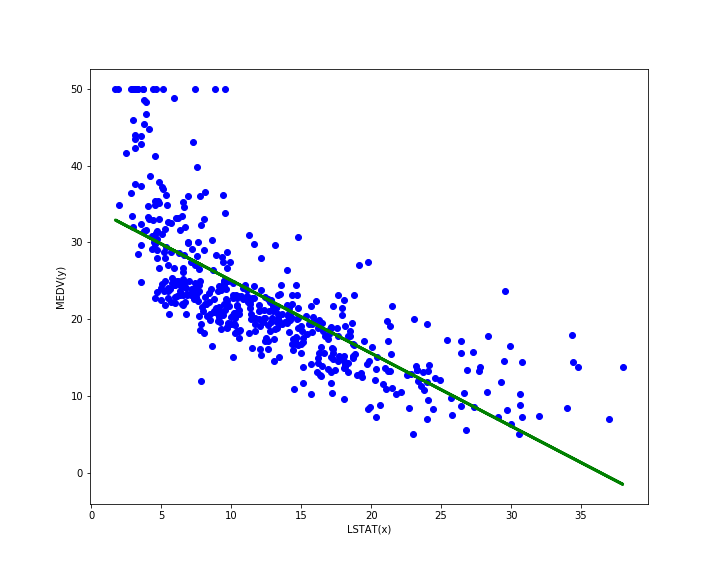
\includegraphics[scale = 0.3]{gradient_descent.png}
	\caption{Fitting a linear model}
\end{figure}
\begin{figure}[h!]
	\centering
	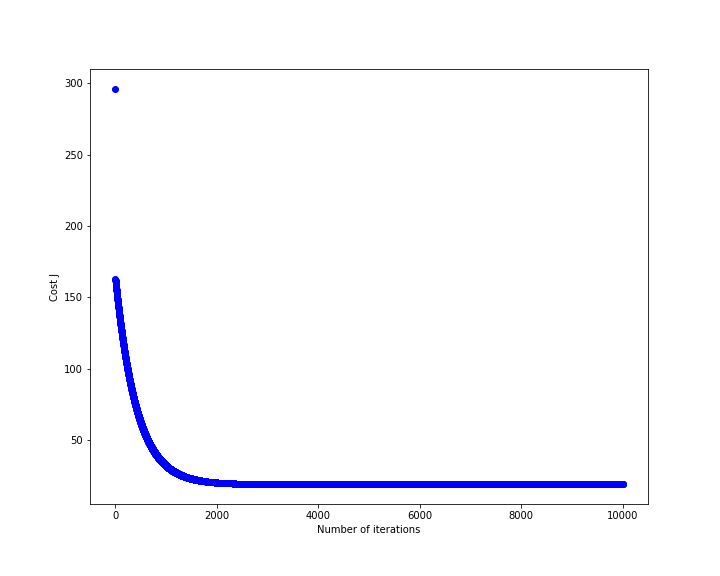
\includegraphics[scale = 0.3]{J_history.png}
	\caption{Convergence of gradient descent}
\end{figure}
    \item A3: Predicting on unseen data\\
    For lower status percentage = 5, we predict a median home value of 298034.49\\
For lower status percentage = 50, we predict a median home value of -129482.13\\
\item B1: Feature normalization\\
\item B2: Loss function and gradient descent\\
\begin{figure}[h!]
	\centering
	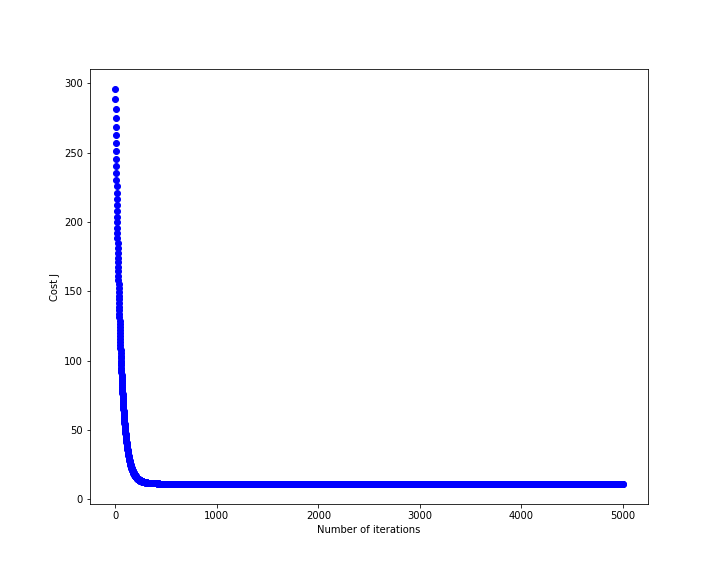
\includegraphics[scale = 0.3]{multi_gradient_descent.png}
	\caption{Convergence of gradient descent with multiple variables}
\end{figure}\\
\item B3: Making predictions on unseen data\\
For average home in Boston suburbs, we predict a median home value of 230467.11\\
\item B4: Normal equations\\
Theta computed by direct solution is: $[ 3.64594884e+01 -1.08011358e-01  4.64204584e-02  2.05586264e-02
  2.68673382e+00 -1.77666112e+01  3.80986521e+00  6.92224640e-04
 -1.47556685e+00  3.06049479e-01 -1.23345939e-02 -9.52747232e-01
  9.31168327e-03 -5.24758378e-01]$\\
For average home in Boston suburbs, we predict a median home value of 230406.54.\\
\pagebreak
\item B5: Exploring convergence of gradient descent
\begin{figure}[htbp]
    \centering
    \subfloat[learning rate=0.01]
    {
    \begin{minipage}[t]{0.5\textwidth}
    \centering
    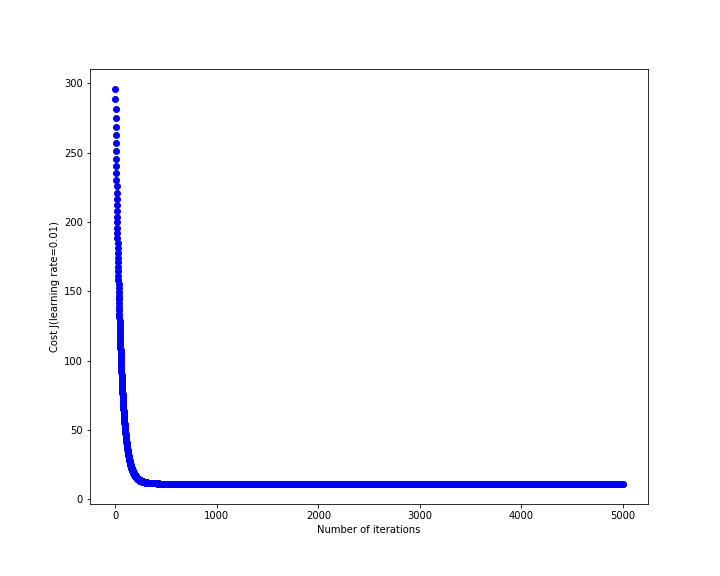
\includegraphics[width=1.0\textwidth]{learning_rate0.png}
    \end{minipage}
    }
    \subfloat[learning rate=0.03]
    {
    \begin{minipage}[t]{0.5\textwidth}
    \centering
    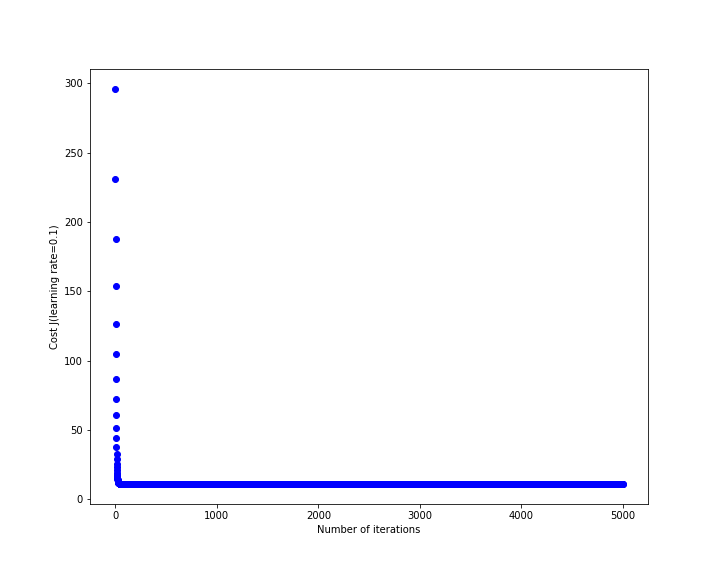
\includegraphics[width=1.0\textwidth]{learning_rate2.png}
    \end{minipage}
    }
    
    \subfloat[learning rate=0.1]
    {
    \begin{minipage}[t]{0.5\textwidth}
    \centering
    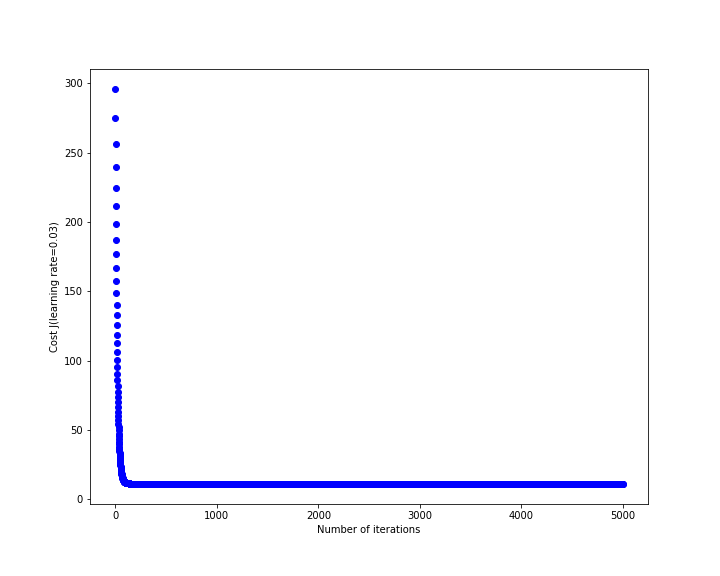
\includegraphics[width=1.0\textwidth]{learning_rate1.png}
    \end{minipage}
    }
    \subfloat[learning rate=0.3]
    {
    \begin{minipage}[t]{0.5\textwidth}
    \centering
    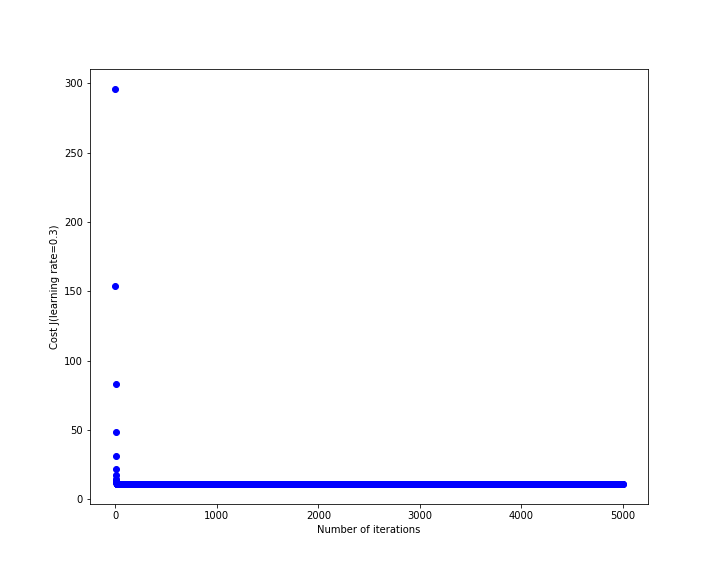
\includegraphics[width=1.0\textwidth]{learning_rate3.png}
    \end{minipage}
    }
    \caption{Convergence of gradient descent with multiple variables according to different learning rates}
\end{figure}

According to the above figures, when learning $rate = 0.01$ is a good choice.\\
\pagebreak

When learning rate = 0.01, chosing different iteration times.\\
\begin{figure}[htbp]
    \centering
    \subfloat[iteration time = 50]
    {
    \begin{minipage}[t]{0.5\textwidth}
    \centering
    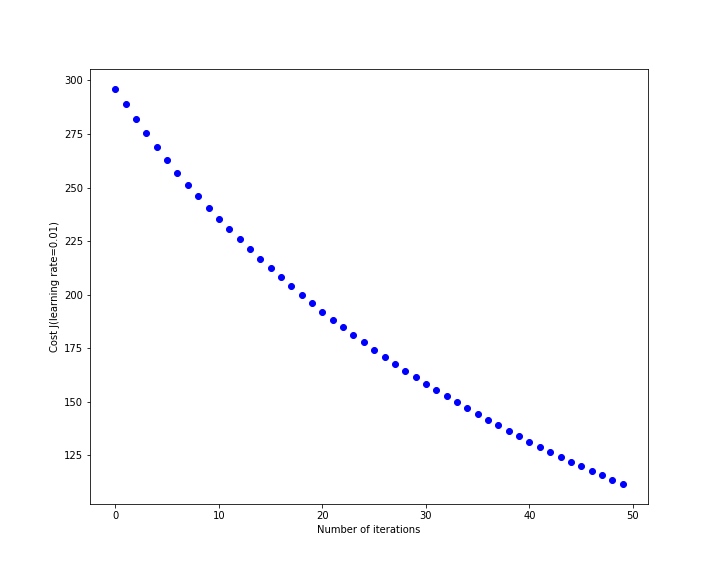
\includegraphics[width=1.0\textwidth]{num_iters0.png}
    \end{minipage}
    }
    \subfloat[iteration time = 500]
    {
    \begin{minipage}[t]{0.5\textwidth}
    \centering
    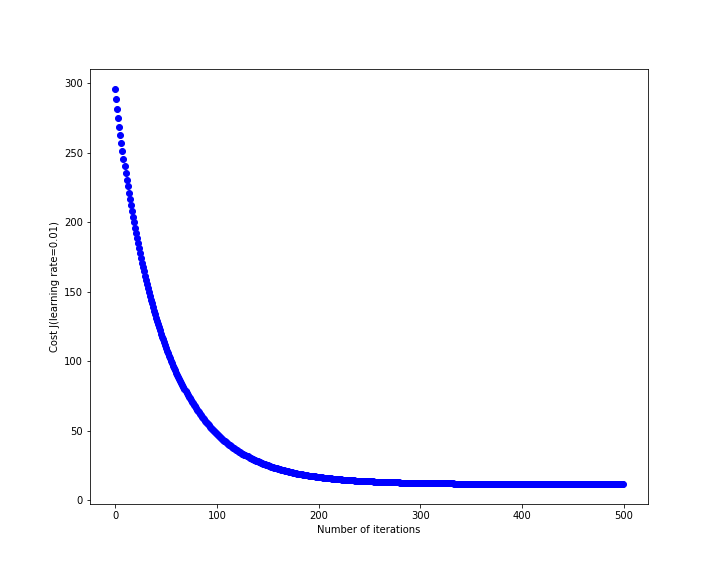
\includegraphics[width=1.0\textwidth]{num_iters1.png}
    \end{minipage}
    }
    
    \subfloat[iteration time = 5000]
    {
    \begin{minipage}[t]{0.5\textwidth}
    \centering
    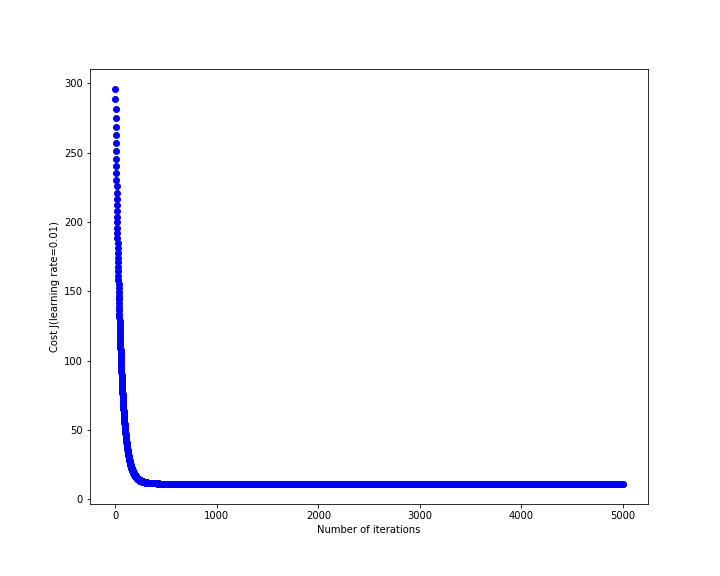
\includegraphics[width=1.0\textwidth]{num_iters2.png}
    \end{minipage}
    }
    \subfloat[iteration time = 50000]
    {
    \begin{minipage}[t]{0.5\textwidth}
    \centering
    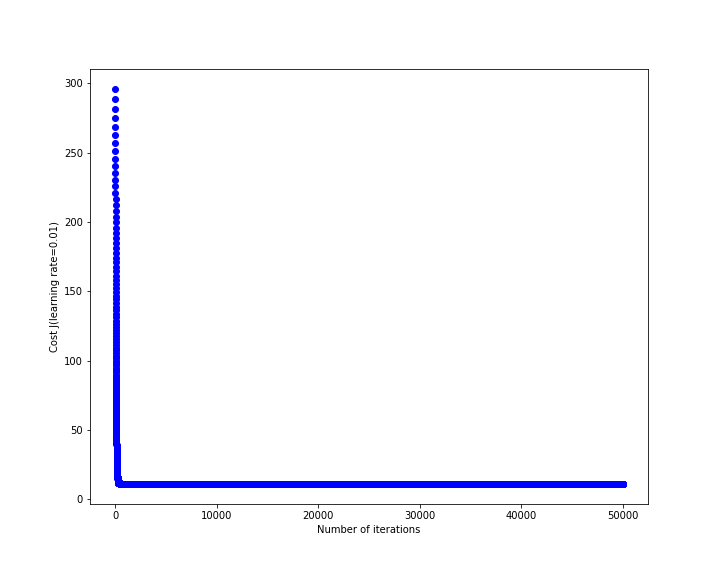
\includegraphics[width=1.0\textwidth]{num_iters3.png}
    \end{minipage}
    }
    \caption{Convergence of gradient descent with multiple variables according to different iteration times}
\end{figure}

According to the above figures, iteration time is 500 is a good choice.
\end{itemize}
\end{document}